% Chapter Template

\chapter{Project Management} % Main chapter title

\label{Chapter2} % Change X to a consecutive number; for referencing this chapter elsewhere, use \ref{ChapterX}

\lhead{Chapter 2. \emph{Project Management}} % Change X to a consecutive number; this is for the header on each page - perhaps a shortened title

%----------------------------------------------------------------------------------------
%	SECTION 1
%----------------------------------------------------------------------------------------

The first section of this chapter introduces the people that made this project possible whereas the following two describe the organizations they represent, Exatronic Innovation Insight and Electronics and Instrumentation Group (GEI).

The last section regards the forseen and final project scheduling.

\section{Context}

This document is intended to report the project developed within the discipline of Project in the school year 2012/2013, which will be submitted to the Faculty of Science and Technologies of the University of Coimbra (FCTUC) to obtain a Master's degree in Biomedical Engineering.

Apart from the FCTUC, where the student was during the first semester, the project was developed along with a portuguese company, Exatronic Insight Innovation, where the student was during the second semester.

The stakeholders responsible for implementation of the project are described in Table \ref{tab:Team}.

% Please add the following required packages to your document preamble:
% 
\begin{table}[h]
\begin{tabular}{@{}ccc@{}}
\toprule
Name&Function& Contact \\ \midrule

 André Carvalheira & Student responsible for & andre.carvalheira1@gmail.com \\
&the execution of the project&\\ \\

Prof. Carlos Correia & Supervisor of the project & correia@fis.uc.pt            \\
&at FCTUC&\\ \\

Eng. André Santos & Supervisor of the project & asantos@exatronic.pt     \\
&at Exatronic Innovation Insight  &\\ \\

Eng. Manuel Loureiro & Supervisor of the project   & mloureiro@exatronic.pt       \\ 
&at Exatronic Innovation Insight&\\ \\

Prof. Miguel Morgado & Coordinator of the projects   & miguel@fis.uc.pt \\
&of the Integrated Masters& \\ 
&in Biomedical Engineering&\\  \midrule
           
\end{tabular}
\caption[Stakeholders]{Stakeholders responsible for implementation of the project}
\label{tab:Team}
\end{table}


\section{Exatronic Innovation Insight}

Exatronic Innovation Insight is a leading Portuguese company in integrated electronics products and solutions.

With 20 years of experience it also creates solutions in product certification and engineering, raw material procurement, sub-contracting production automation and automotive section.

Since 2010 a new business area was created, Exa4Life, which fits this project through an established protocol with the University of Coimbra, the University of Aveiro and Instituto Superior Técnico.

Experience - electrotherapy, ECG

\section{Electronics and Instrumentation Group (GEI)}

Thr Electronics and Instrumentation Group (Grupo de Electrónica e Instrumentação, GEI) is based in the Physics Department of the University of Coimbra. 

The research areas of the Electronics and Instrumentation Group (GEI) are Atomic and Nuclear Instrumentation, Biomedical Instrumentation, Plasma Physics Instrumentation, Microelectronics, Optical Signal Processing and Telemetry and Industrial Control.

The GEI keeps a close cooperation with several national and international institutions that develop work in common research areas with unquestionable scientific results. 

Concerning the teaching practice, GEI strongly supports the Instrumentation branch of the Physics Engineering degree and Biomedical Engineering degree with all its specialization branches. 

This center has great deal of concern with the community services promoted during the last years by regular cooperation with several national companies, consulting services, conference participation, symposia as well as the coordination of several Ciência Viva projects promoted by the National Science and Technology National Ministry.

\section{Schedule}

The project schedule was done using a Gantt diagram. 

Figure \ref{fig:Gantt} shows the Gantt diagram with the macro tasks proposed by Exatronic and their expected timing.

\begin{figure}[htbp]
\centering
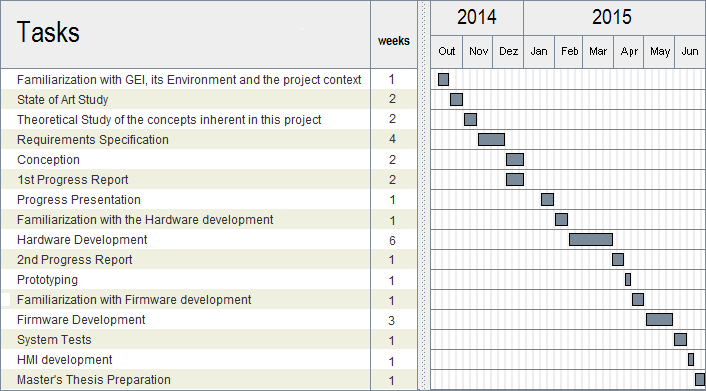
\includegraphics[width=1\textwidth]{Figures/gantt.png}
\caption[Gantt Diagram]{Gantt Diagram of the project.}
\label{fig:Gantt}
\end{figure}